\label{section_results}
We developed a code in Python based on the methods exposed in Section \ref{section_models_maze} for assessing our algorithm's performance. Pseudocode \ref{pseudocode_1} and Pseudocode \ref{pseudocode_2} guided the reasoning behind the code, that is available on \href{https://github.com/ArthurJose2000/mazeexploration}{github.com/ArthurJose2000/mazeexploration}.

This work used perfect mazes for simulating multi-agent scenarios where agents go through the mazes in order to find the goal. Section \ref{section_results_our_performance} presents the agents's performance when they use our algorithm. Section \ref{section_results_incremental_policy} proposes an agent policy modification when it finishes its interval for improving its performance. Finally Section \ref{section_results_tarry_vs_our} compares our algorithm's performance to the performance of the extended Tarry's algorithm \cite{KivelevitchCohen2010}, despite the latter having communication between agents.

\section{Our algorithm's perfomance}
\label{section_results_our_performance}

In order to assess our algotihm's performance, this work generates, using the code provided by \citen{Muhammad2021}, 250 random and perfect mazes for each type of size - $10 \times 10$, $20 \times 20$, $30 \times 30$, and $40 \times 40$. As they are perfect mazes, i.e., there is only one path to the goal from any cell, any node of the maze's tree representation has the same convergence interval for every agent. Thus, the developed code aims to fill the concept of dispersion, where the agents try to go through the maze as dispersed as possible without communication.

For each maze size, the code ran 1 single agent until 40 cooperative agents going through 250 different mazes, since this work generated 250 random perfect mazes for each type of size. In order to analyse the results, the authors computed the following classes of analysis:

\begin{itemize}
\item Average of steps: the average of steps of one agent in each maze, where the total number of steps is divided by the number of agents.

\item Pioneer's average of steps: the average of steps of the first agent that reaches the goal, i.e., the pioneer.

\item STDEV - Average of steps: the standard deviation of the average of steps of one agent considering all the 250 different mazes.

\item Fraction of maze explored: the percentage of visited cells until every agent stops.

\item Fraction of maze explored when pioneer reaches target: the percentage of visited cells at the moment when the pioneer reaches the goal.
\end{itemize}

As pointed out in Section \ref{section_models_exploration_key_concepts}, where the key concepts of this research are exposed, it is worth emphasizing that some agents doesn't find the goal, so it is possible that some agent stops the search before the pioneer finds the goal. It is clearer for big mazes, as seem in Figure \ref{our_algorithm_steps_40_x_40}, where in some situations the average of steps is smaller than the pioneer's average of steps, that might seem incoherent at first looking. If the approach of Pseudocode \ref{pseudocode_1} is modified so that each agent must find the goal after fills its interval, obviously the average of steps must be bigger than the pioneer's average of steps.

Figure \ref{our_algorithm_steps} presents, for each maze size - $10 \times 10$, $20 \times 20$, $30 \times 30$, and $40 \times 40$ -, the results of average of steps, pioneer's average of steps, and standard deviation of the average of steps considering all the 250 different mazes. Similarly, Figure \ref{our_algorithm_fraction} presents the results of fraction of explored maze and fraction of maze explored when pioneer reaches the target.

\begin{figure}
    \centering
    \subfloat[\centering $10 \times 10$ maze]
    {{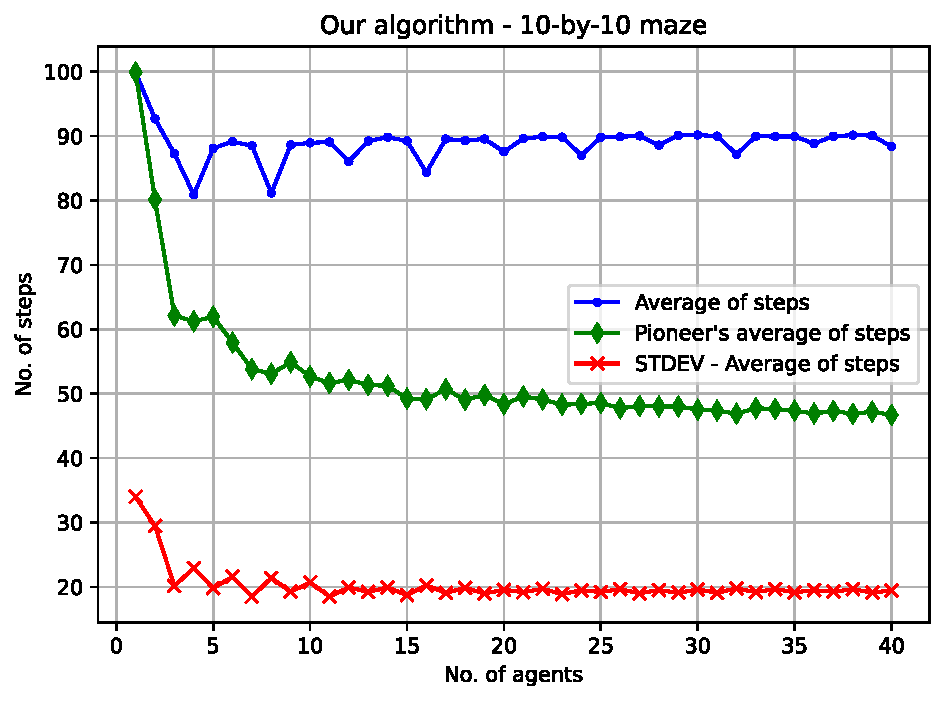
\includegraphics[width=.45\linewidth]{Cap3/our_algorithm/our_algorithm_10x10_steps.pdf} }}
    \qquad
    \subfloat[\centering $20 \times 20$ maze]
    {{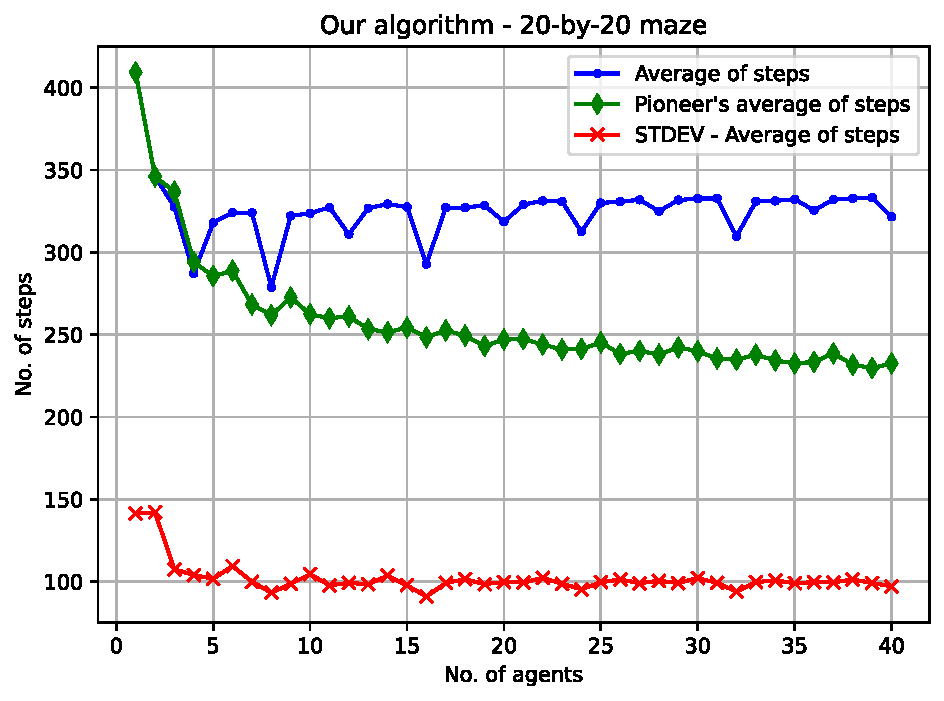
\includegraphics[width=.45\linewidth]{Cap3/our_algorithm/our_algorithm_20x20_steps.pdf} }}
    \qquad
    \newline
    \subfloat[\centering $30 \times 30$maze]
    {{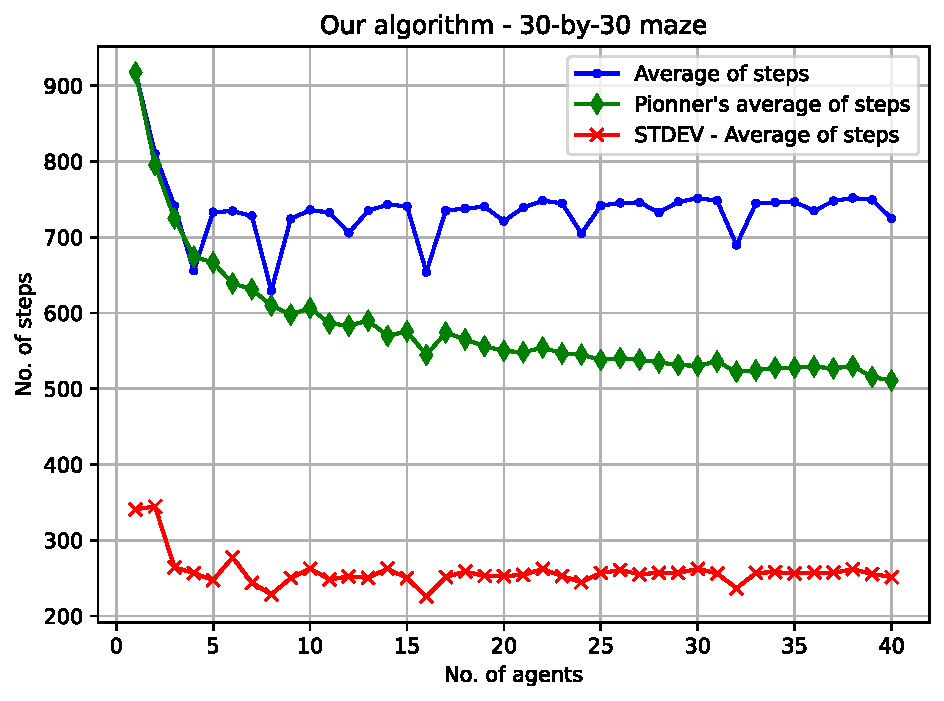
\includegraphics[width=.45\linewidth]{Cap3/our_algorithm/our_algorithm_30x30_steps.pdf} }}
    \qquad
    \subfloat[\centering $40 \times 40$maze]
    {{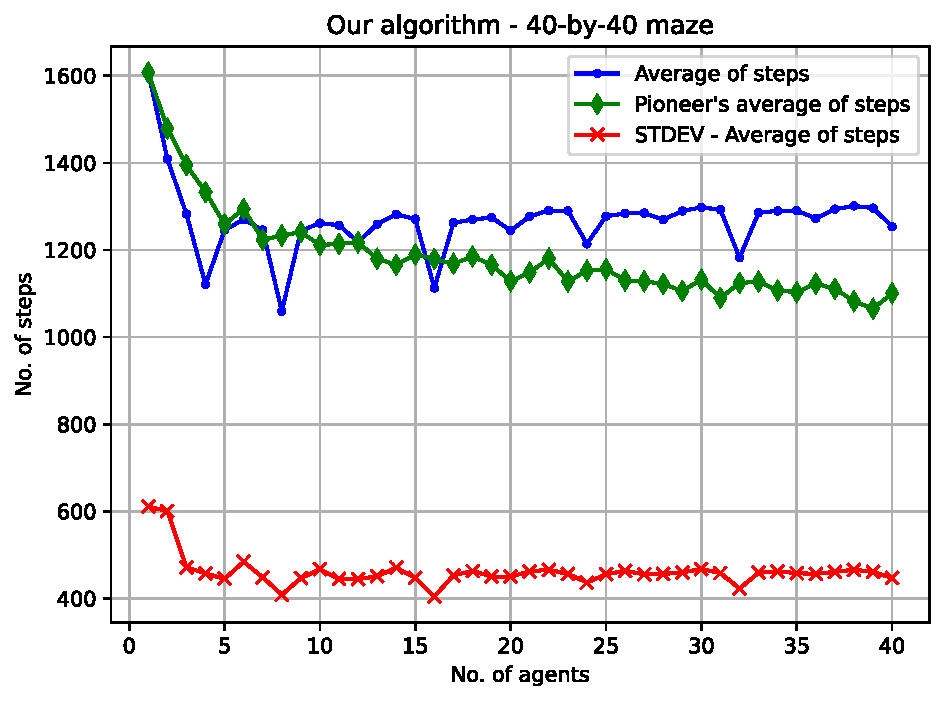
\includegraphics[width=.45\linewidth]{Cap3/our_algorithm/our_algorithm_40x40_steps.pdf}
    \label{our_algorithm_steps_40_x_40} }}
    \caption{Results of average of steps, pioneer's average of steps, and standard deviation of the average of steps. 1 single agent until 40 cooperative agents were run in 250 different mazes for each type of size.}
    \label{our_algorithm_steps}
\end{figure}

\begin{figure}
    \centering
    \subfloat[\centering $10 \times 10$ maze]
    {{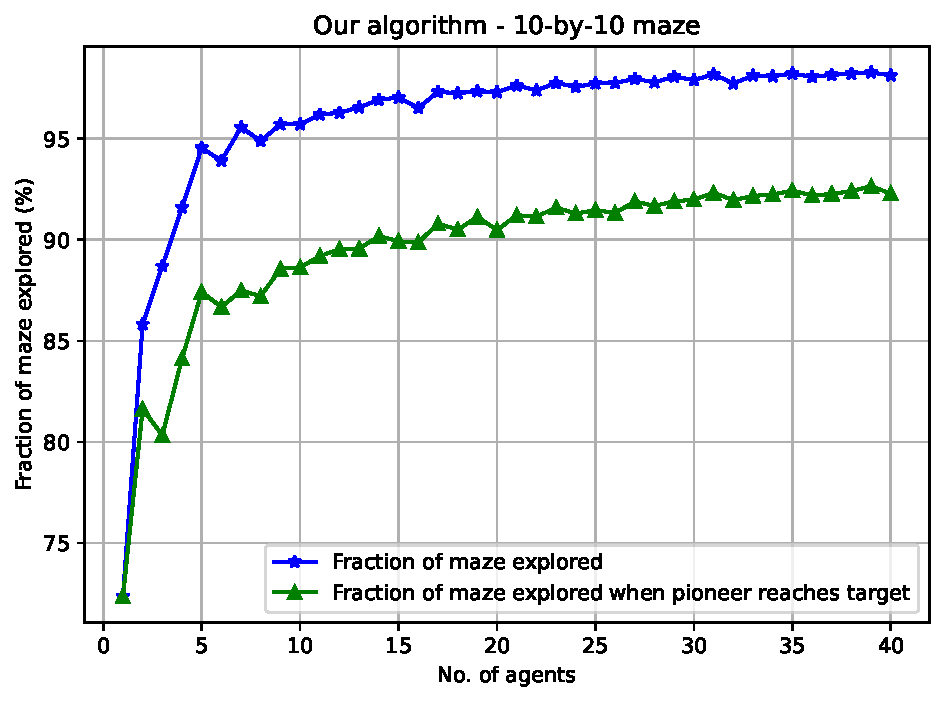
\includegraphics[width=.45\linewidth]{Cap3/our_algorithm/our_algorithm_10x10_fraction.pdf} }}
    \qquad
    \subfloat[\centering $20 \times 20$ maze]
    {{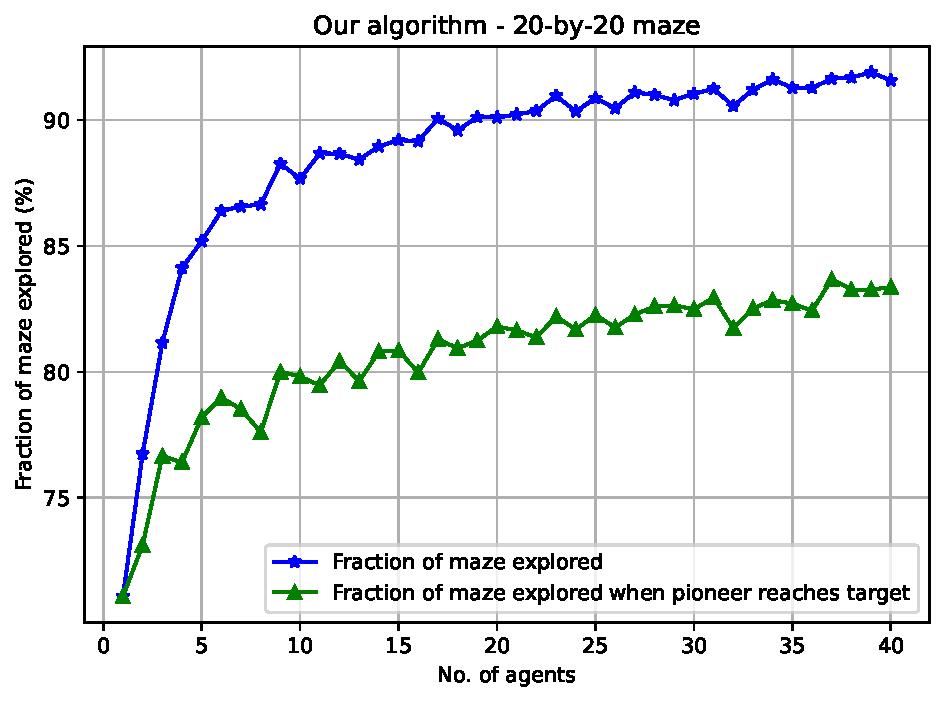
\includegraphics[width=.45\linewidth]{Cap3/our_algorithm/our_algorithm_20x20_fraction.pdf} }}
    \qquad
    \newline
    \subfloat[\centering $30 \times 30$maze]
    {{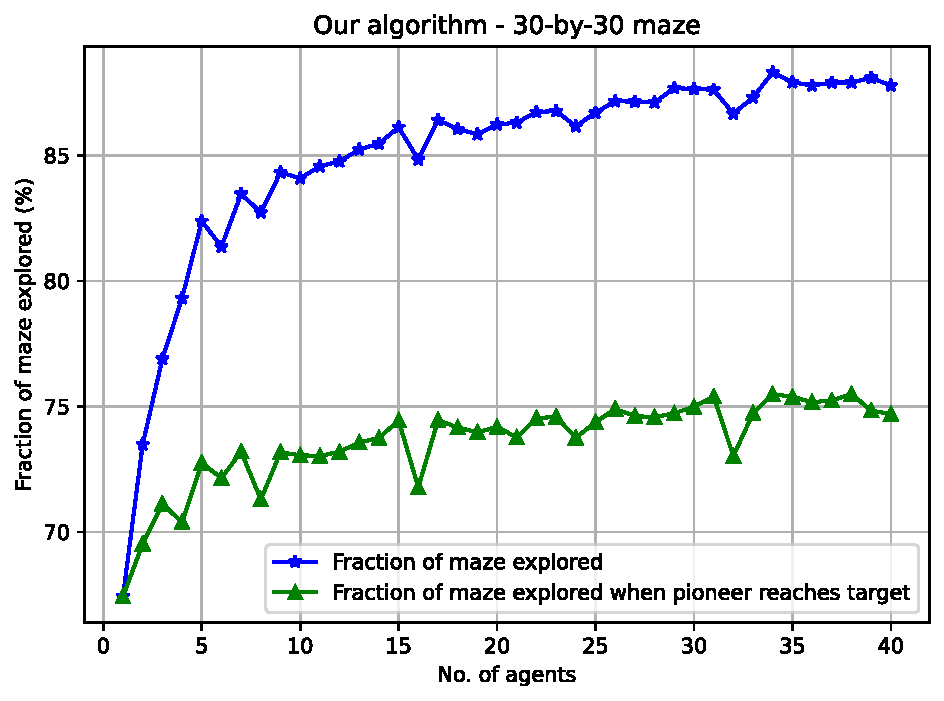
\includegraphics[width=.45\linewidth]{Cap3/our_algorithm/our_algorithm_30x30_fraction.pdf} }}
    \qquad
    \subfloat[\centering $40 \times 40$maze]
    {{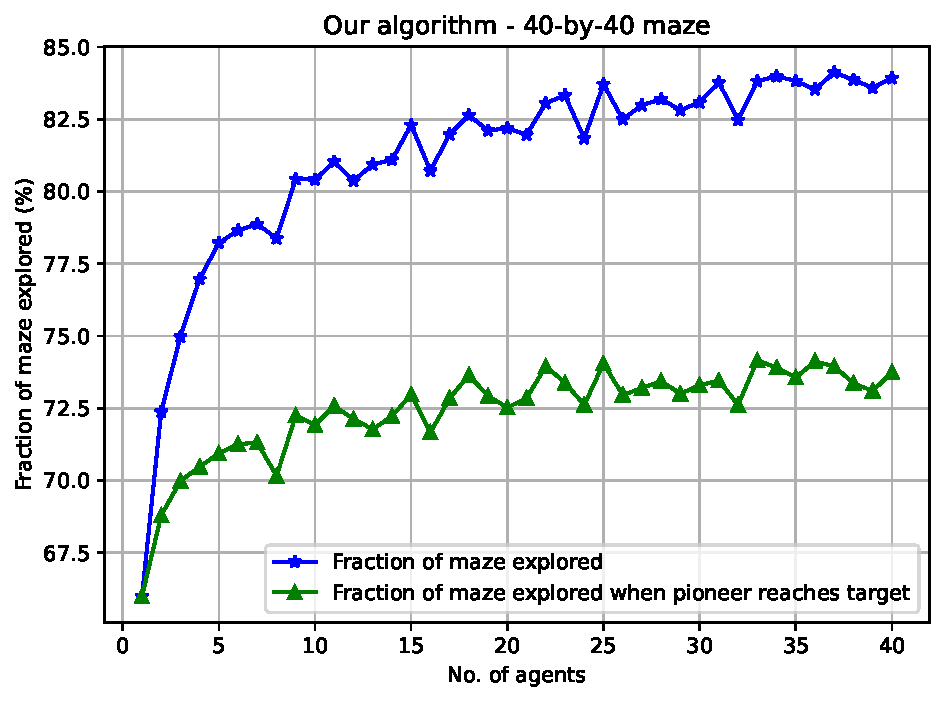
\includegraphics[width=.45\linewidth]{Cap3/our_algorithm/our_algorithm_40x40_fraction.pdf} }}
    \caption{Results of fraction of explored maze and fraction of maze explored when pioneer reaches the target. 1 single agent until 40 cooperative agents were run in 250 different mazes for each type of size.}
    \label{our_algorithm_fraction}
\end{figure}


\section{Incremental policy for the agents}
\label{section_results_incremental_policy}

After establishing an algorithm where the agents focus to fill its interval, this work implemented a slight modification, where the agent change its interval and its order of action after finishing its starting interval.

As pointed out in Pseudocode \ref{pseudocode_1}, the order of action of each agent is clockwise in the context of maze - North, East, South, and West. Supposing that there are $k$ agents $a_{1}, a_{2},...,a_{k}$ to explore the maze, there will be $k$ different acting intervals, as seen in Equation \ref{equation_agent_intervals}. With our incremental policy, when the agent $a_{i}$ finishes its interval, its interval gets the value of the starting interval of $a_{i+1}$ if $i < k$. If $i = k$, it gets the value of the starting interval of $a_{0}$. Furthermore, the agent changes its order of action from clockwise to counter-clockwise - West, South, East, and North -, i.e, from right to left relating to the order of children.

Figure \ref{tree_example_incremental_policy} gives an example of such incremental policy, where an agent with interval $[0, \frac{1}{3}[$ finishes its interval in the 5th node, and then it changes its interval to $[\frac{1}{3}, \frac{2}{3}[$, and changes the order of action from left-right to right-left.

Figures \ref{our_algorithm_1I_vs_2I_steps} and \ref{our_algorithm_1I_vs_2I_fraction} present the comparison between our ``1 interval'' algorithm - evaluated in Section \ref{section_results_our_performance} - and our ``2 intervals'' algorithm, where the incremental policy was implemented.

The first conclusion that can taken from the incremental is that it improves the search in the sense of amount of steps the a pioneer must do to reach the target. For instance, as seen in Figure \ref{our_algorithm_1I_vs_2I_steps_40_x_40}, in the context of 40 cooperative agents in $40 \times 40$ mazes, with the incremental policy, the pioneer reaches the target with about 18\% less steps compared to the our ``1 interval'' approach. Moreover, as such policy improves the dispersion, more cells are visited, as seen in Figure \ref{our_algorithm_1I_vs_2I_fraction}.

\begin{figure}[ht!]
\centering
\begin{forest}

%for tree={circle,draw,minimum size=3em,inner sep=1pt,s sep=12mm}

 [1,label=above:{\textit{Starting point}},for tree={circle,draw,minimum size=2em,s sep=12mm},label=below:{$[0,1]$},fill=red!100
 	[2,label=above:{$[0,\frac{1}{3}[$},fill=red!100
 		[3,label=below:{$[0,\frac{1}{9}[$},fill=red!100]
 		[4,label=below:{$[\frac{1}{9},\frac{2}{9}[$},fill=red!100]
 		[5,label=below:{$[\frac{2}{9},\frac{1}{3}[$},fill=red!100]]
 	[6,label=right:{$[\frac{1}{3},\frac{2}{3}]$},fill=red!100
 		[10,label=below:{$[\frac{1}{3},\frac{1}{2}[$},fill=red!100
 		[12,label=below:{$[\frac{1}{3},\frac{5}{12}[$},fill=red!100]
 		[11,label=below:{$[\frac{5}{12},\frac{1}{2}[$},fill=red!100]]
 		[7,label=below:{$[\frac{1}{2},\frac{2}{3}]$},fill=red!100
 			[9,label=below:{$[\frac{1}{2},\frac{7}{12}[$},fill=red!100]
 			[8,label=below:{$[\frac{7}{12},\frac{2}{3}]$},fill=red!100]]]
 	[
 		[$\vdots$,draw=black!0]]]

\end{forest}
\caption{Example of an agent with interval $[0, \frac{1}{3}[$ under the incremental policy, where it changes its interval to $[\frac{1}{3}, \frac{2}{3}[$ when it finishes its starting interval, in the 5th visited cell, and it changes the order of action to right-left.}
\label{tree_example_incremental_policy}
\end{figure}

\begin{figure}
    \centering
    \subfloat[\centering LEEEEEEEGEEEENDDAAA]
    {{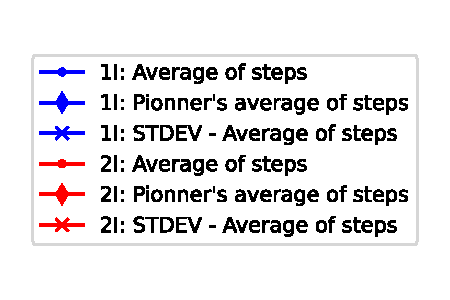
\includegraphics[width=.45\linewidth]{Cap3/our_algorithm_incremental_policy/legend_steps.pdf} }}
    \newline
    \subfloat[\centering $10 \times 10$ maze]
    {{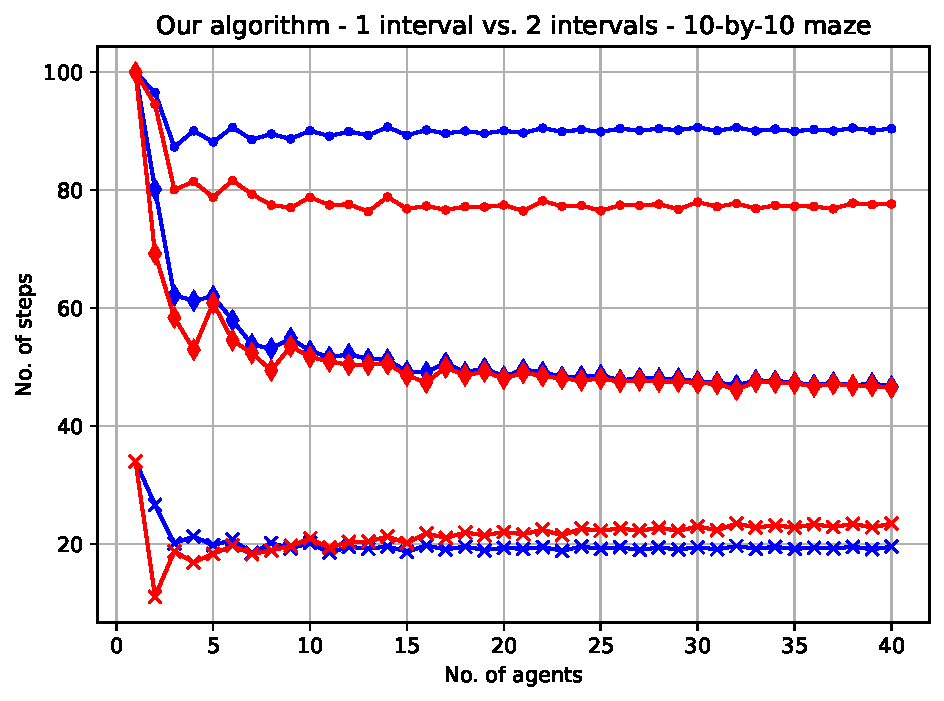
\includegraphics[width=.45\linewidth]{Cap3/our_algorithm_incremental_policy/our_algorithm_1I_vs_2I_10x10_steps.pdf} }}
    \qquad
    \subfloat[\centering $20 \times 20$ maze]
    {{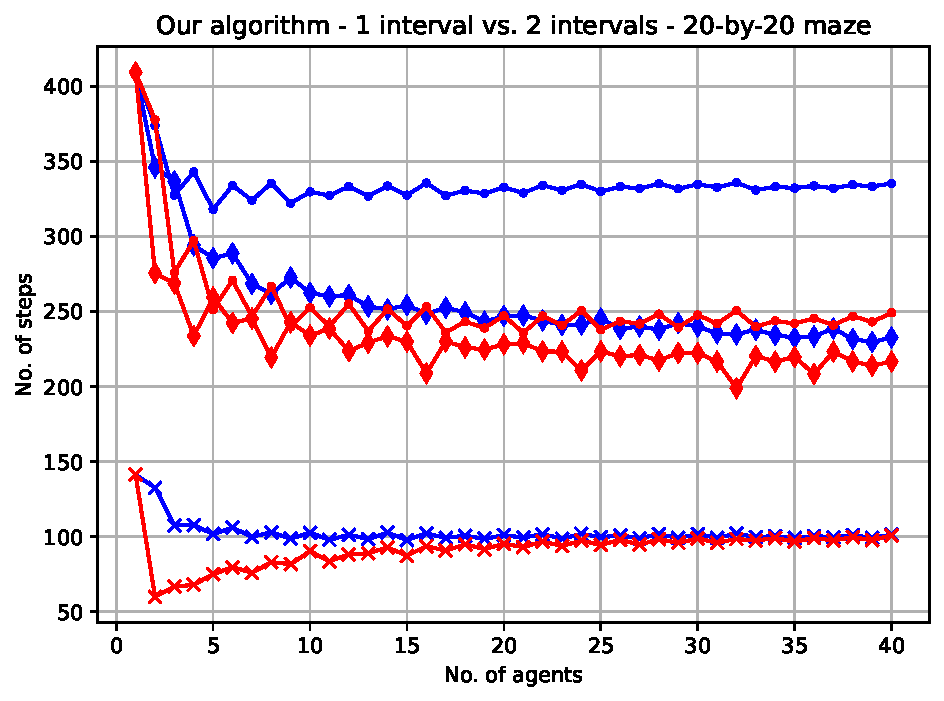
\includegraphics[width=.45\linewidth]{Cap3/our_algorithm_incremental_policy/our_algorithm_1I_vs_2I_20x20_steps.pdf} }}
    \qquad
    \newline
    \subfloat[\centering $30 \times 30$maze]
    {{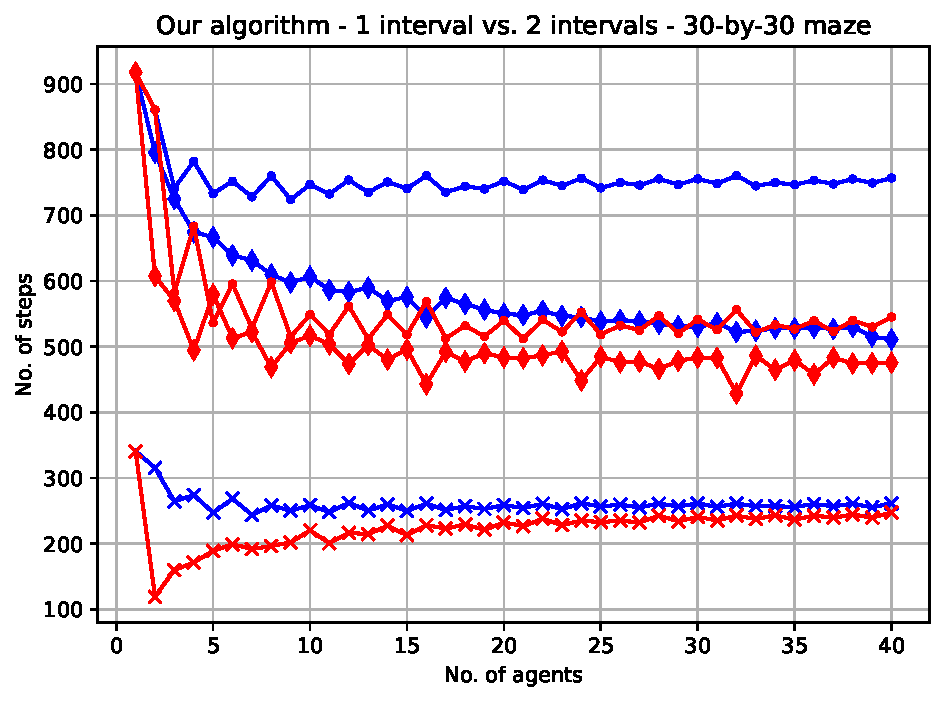
\includegraphics[width=.45\linewidth]{Cap3/our_algorithm_incremental_policy/our_algorithm_1I_vs_2I_30x30_steps.pdf} }}
    \qquad
    \subfloat[\centering $40 \times 40$maze]
    {{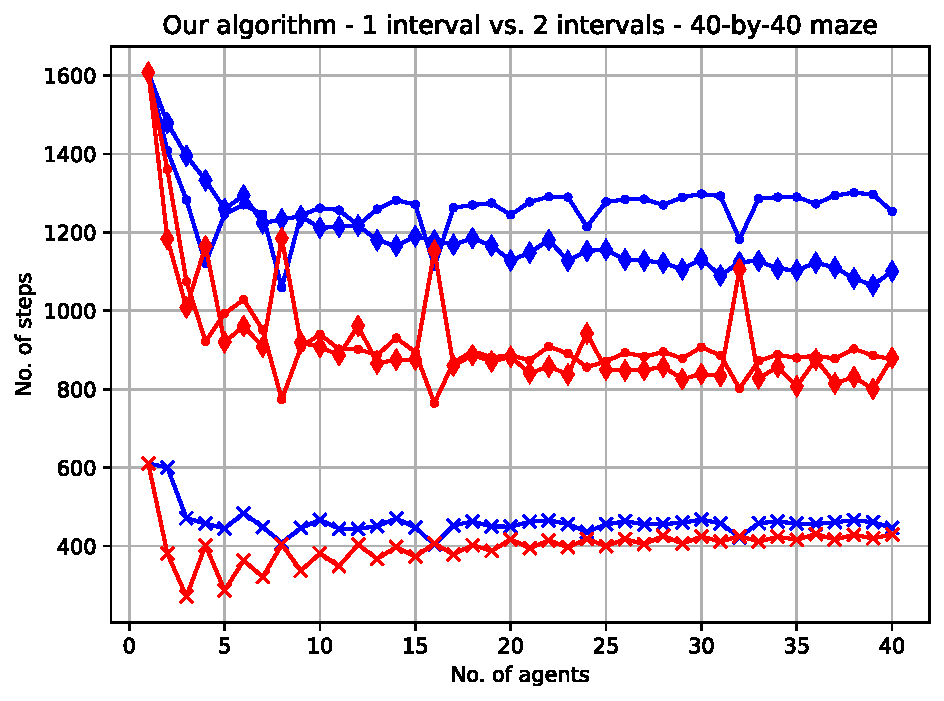
\includegraphics[width=.45\linewidth]{Cap3/our_algorithm_incremental_policy/our_algorithm_1I_vs_2I_40x40_steps.pdf}
    \label{our_algorithm_1I_vs_2I_steps_40_x_40} }}
    \caption{...}
    \label{our_algorithm_1I_vs_2I_steps}
\end{figure}

\begin{figure}
    \centering
    \subfloat[\centering LEEEEEEEGEEEENDDAAA]
    {{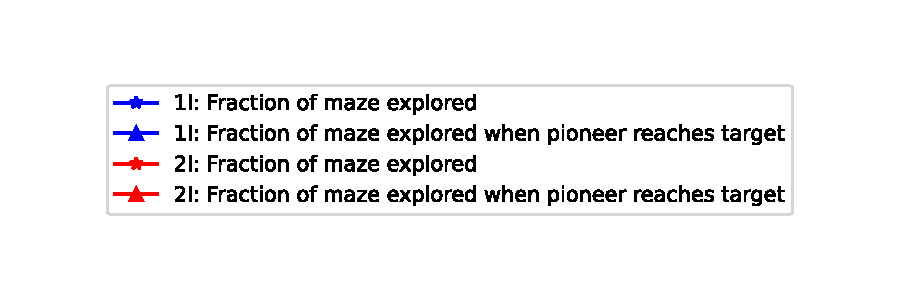
\includegraphics[width=.45\linewidth]{Cap3/our_algorithm_incremental_policy/legend_fraction.pdf} }}
    \newline
    \subfloat[\centering $10 \times 10$ maze]
    {{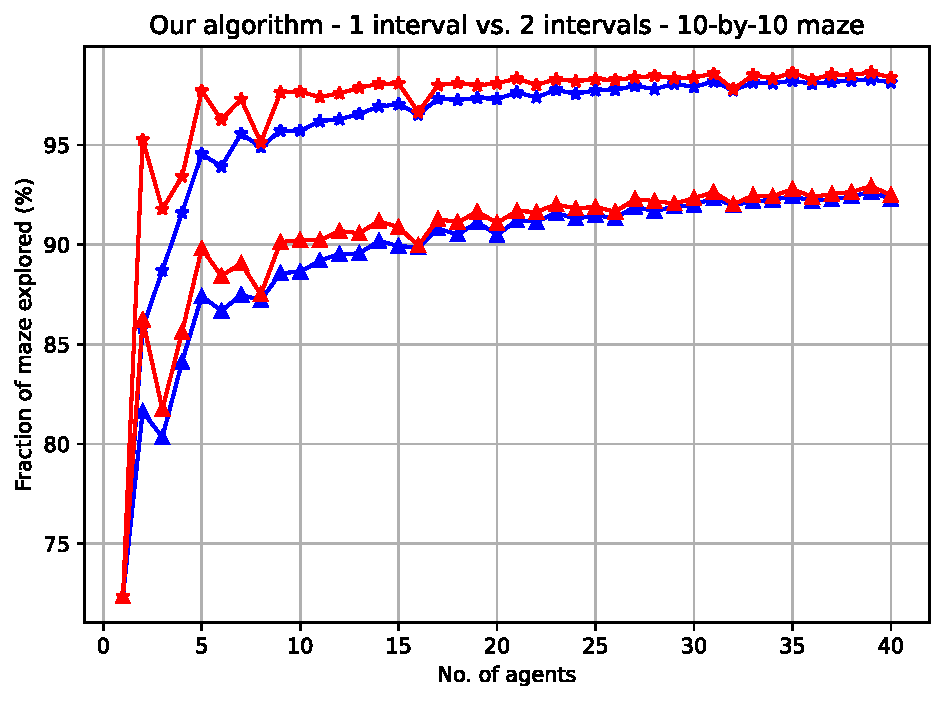
\includegraphics[width=.45\linewidth]{Cap3/our_algorithm_incremental_policy/our_algorithm_1I_vs_2I_10x10_fraction.pdf} }}
    \qquad
    \subfloat[\centering $20 \times 20$ maze]
    {{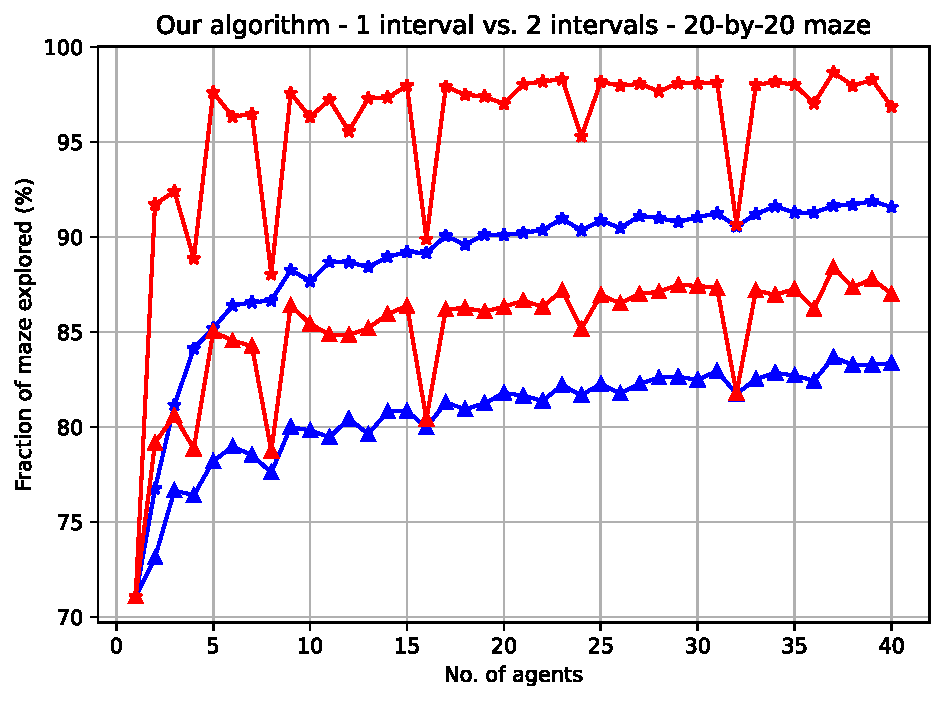
\includegraphics[width=.45\linewidth]{Cap3/our_algorithm_incremental_policy/our_algorithm_1I_vs_2I_20x20_fraction.pdf} }}
    \qquad
    \newline
    \subfloat[\centering $30 \times 30$maze]
    {{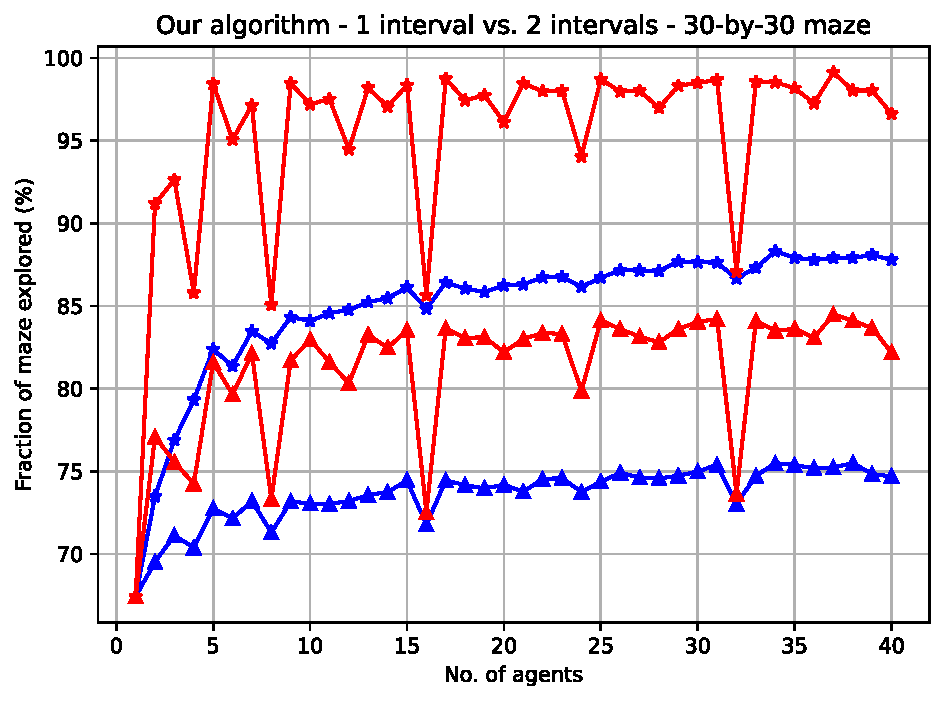
\includegraphics[width=.45\linewidth]{Cap3/our_algorithm_incremental_policy/our_algorithm_1I_vs_2I_30x30_fraction.pdf} }}
    \qquad
    \subfloat[\centering $40 \times 40$maze]
    {{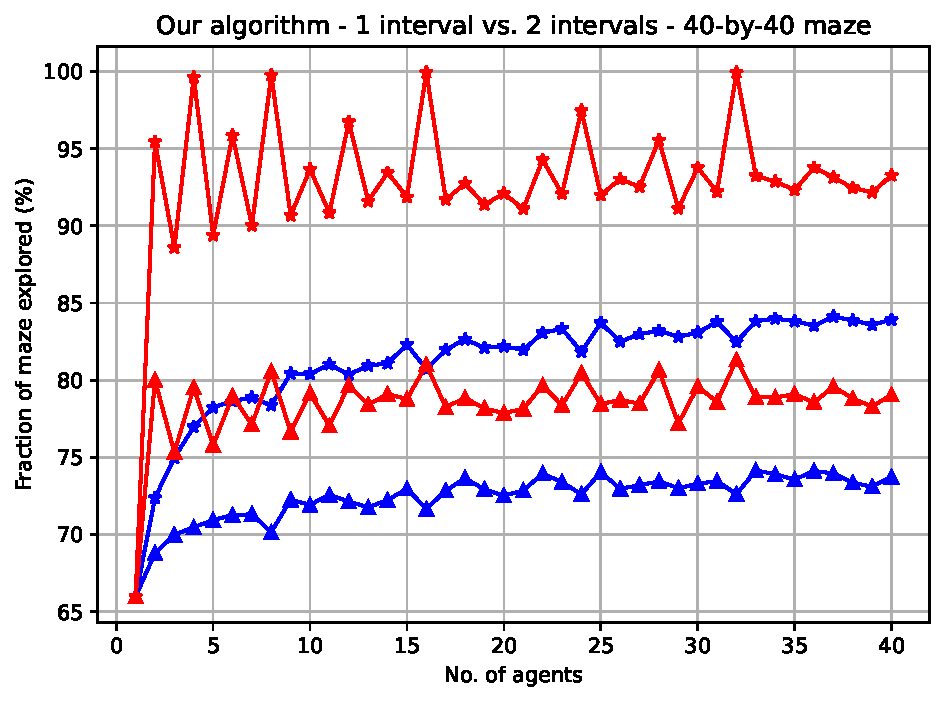
\includegraphics[width=.45\linewidth]{Cap3/our_algorithm_incremental_policy/our_algorithm_1I_vs_2I_40x40_fraction.pdf} }}
    \caption{...}
    \label{our_algorithm_1I_vs_2I_fraction}
\end{figure}

\section{Our algorithm vs. Tarry's algorithm}
\label{section_results_tarry_vs_our}

\begin{figure}
    \centering
    \subfloat[\centering $10 \times 10$ maze]
    {{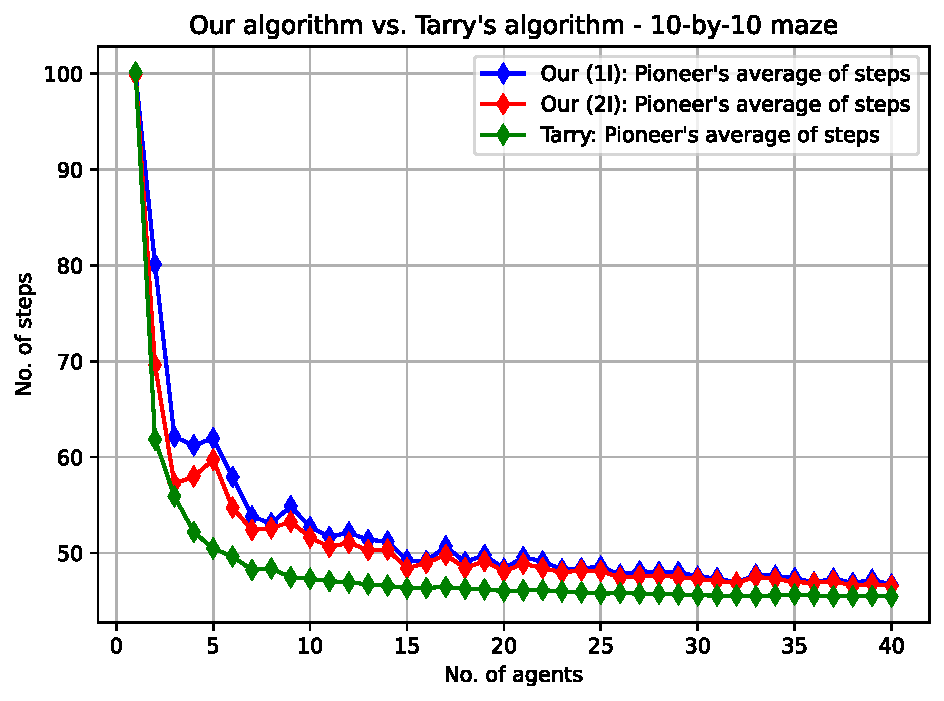
\includegraphics[width=.45\linewidth]{Cap3/our_algorithm_vs_tarry_algorithm/our_algorithm_vs_tarry_10x10_steps.pdf} }}
    \qquad
    \subfloat[\centering $20 \times 20$ maze]
    {{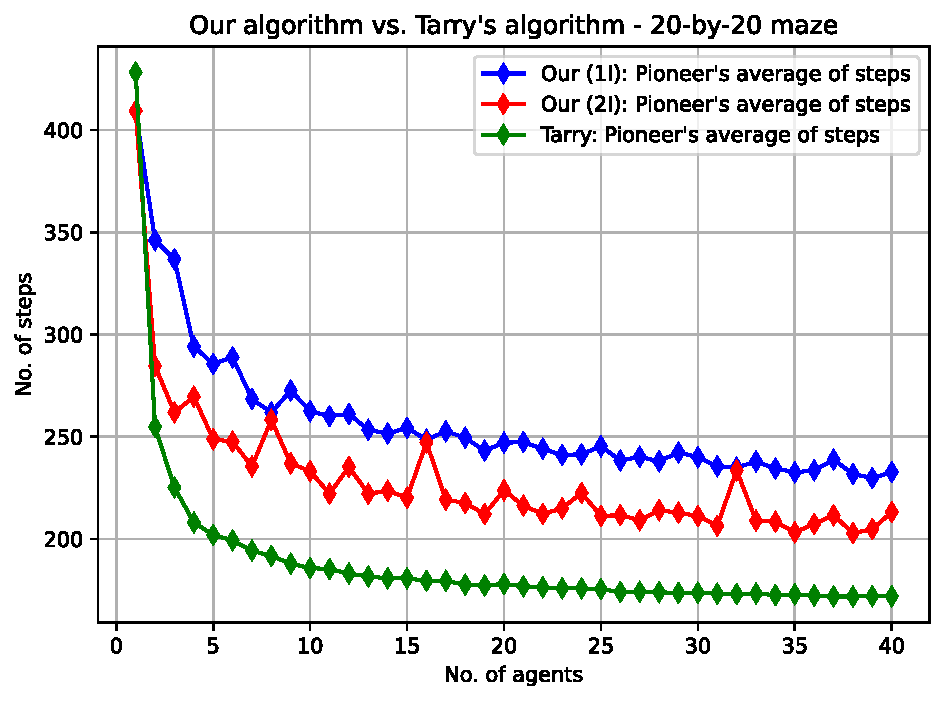
\includegraphics[width=.45\linewidth]{Cap3/our_algorithm_vs_tarry_algorithm/our_algorithm_vs_tarry_20x20_steps.pdf} }}
    \qquad
    \newline
    \subfloat[\centering $30 \times 30$maze]
    {{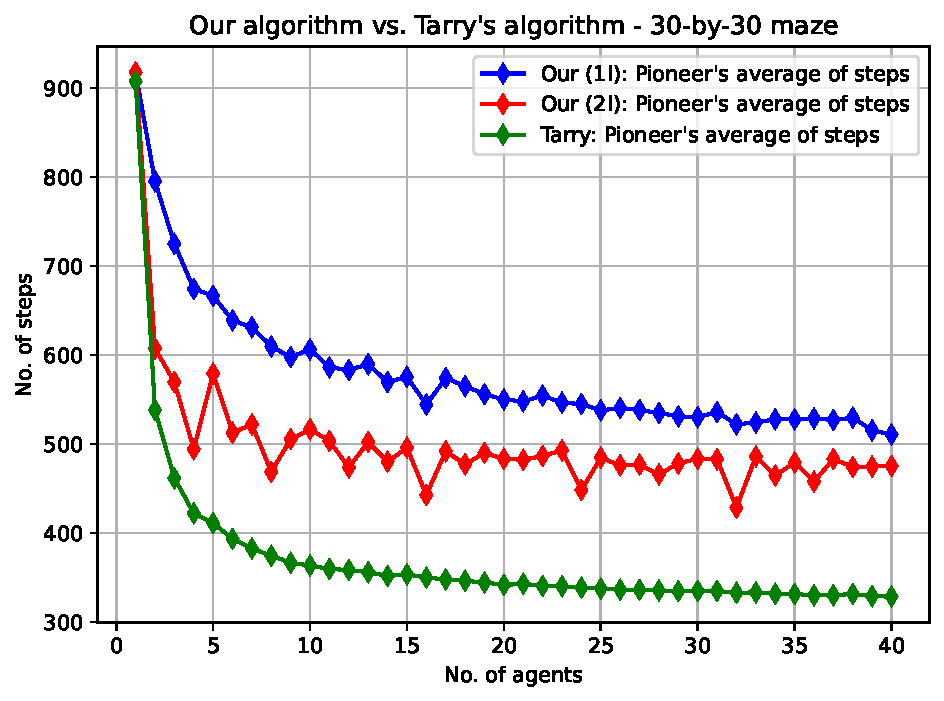
\includegraphics[width=.45\linewidth]{Cap3/our_algorithm_vs_tarry_algorithm/our_algorithm_vs_tarry_30x30_steps.pdf} }}
    \qquad
    \subfloat[\centering $40 \times 40$maze]
    {{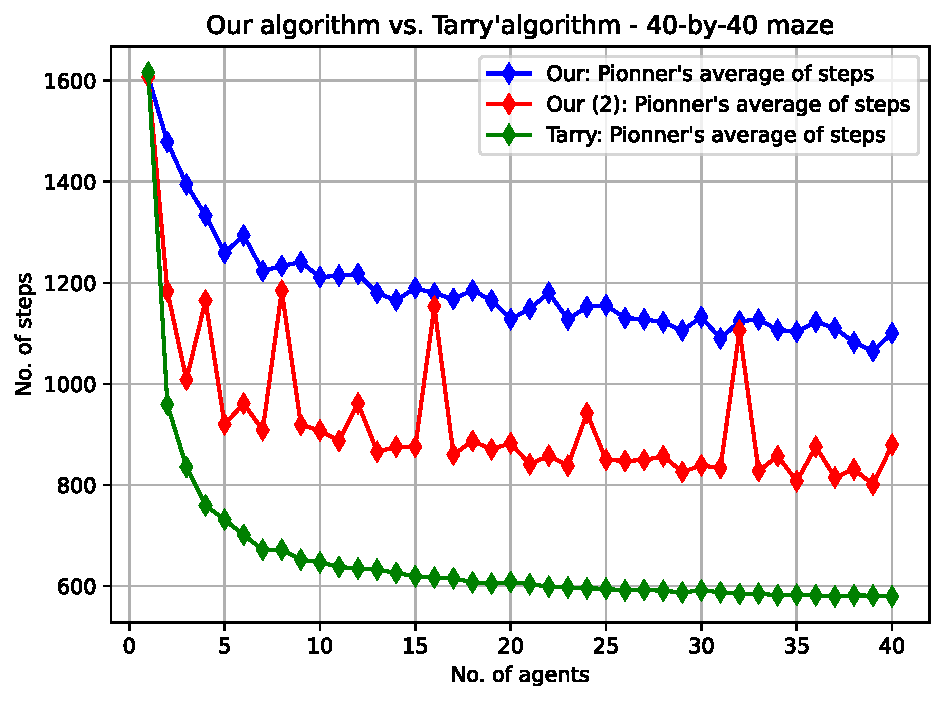
\includegraphics[width=.45\linewidth]{Cap3/our_algorithm_vs_tarry_algorithm/our_algorithm_vs_tarry_40x40_steps.pdf} }}
    \caption{...}
    \label{our_algorithm_vs_tarry_steps}
\end{figure}

\begin{figure}
    \centering
    \subfloat[\centering $10 \times 10$ maze]
    {{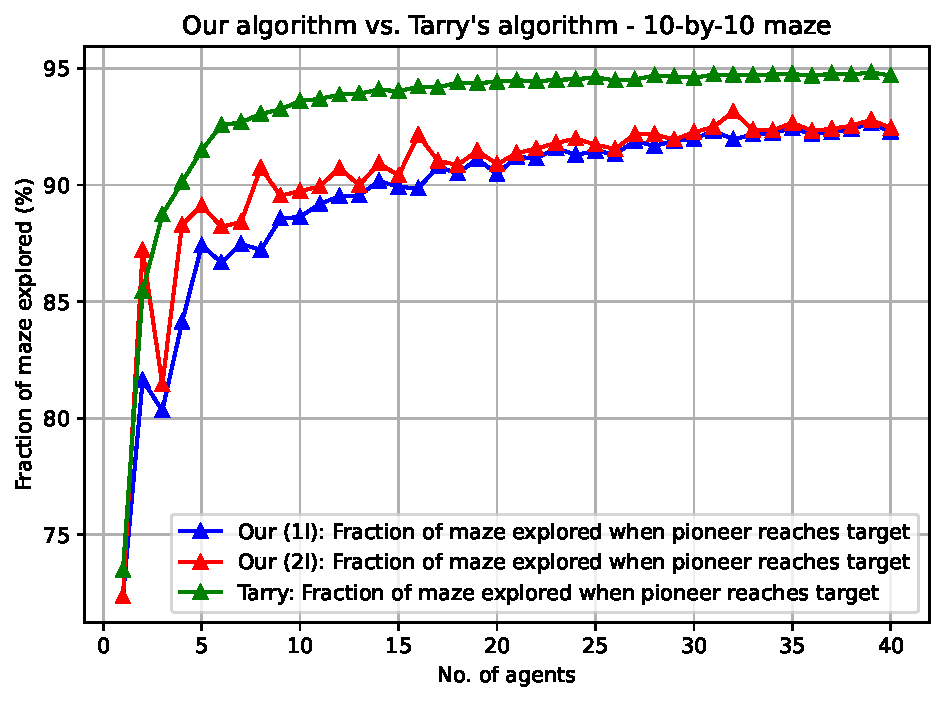
\includegraphics[width=.45\linewidth]{Cap3/our_algorithm_vs_tarry_algorithm/our_algorithm_vs_tarry_10x10_fraction.pdf} }}
    \qquad
    \subfloat[\centering $20 \times 20$ maze]
    {{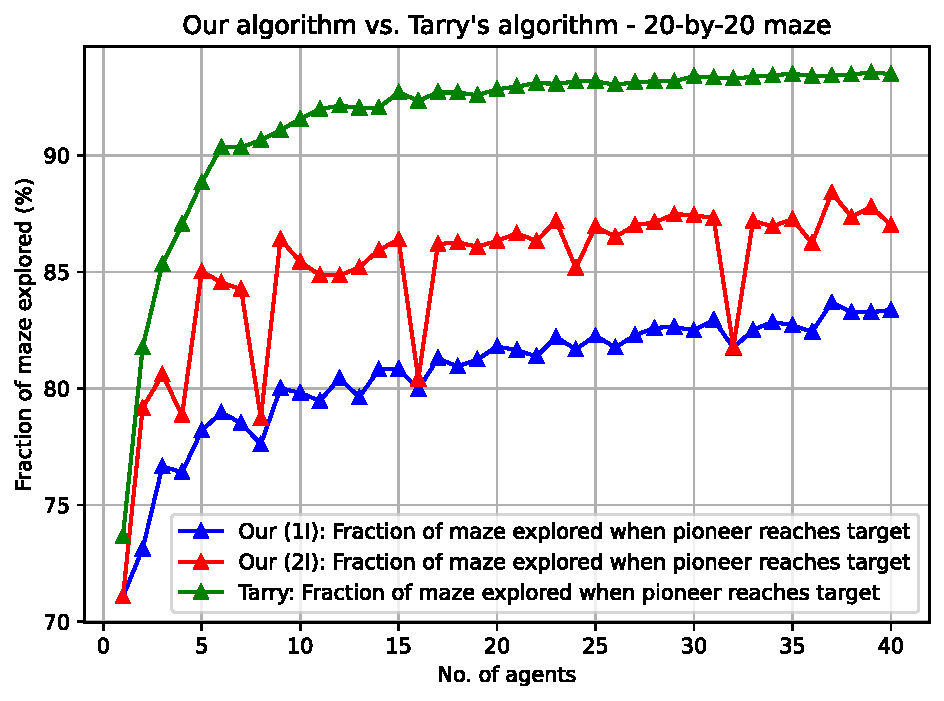
\includegraphics[width=.45\linewidth]{Cap3/our_algorithm_vs_tarry_algorithm/our_algorithm_vs_tarry_20x20_fraction.pdf} }}
    \qquad
    \newline
    \subfloat[\centering $30 \times 30$maze]
    {{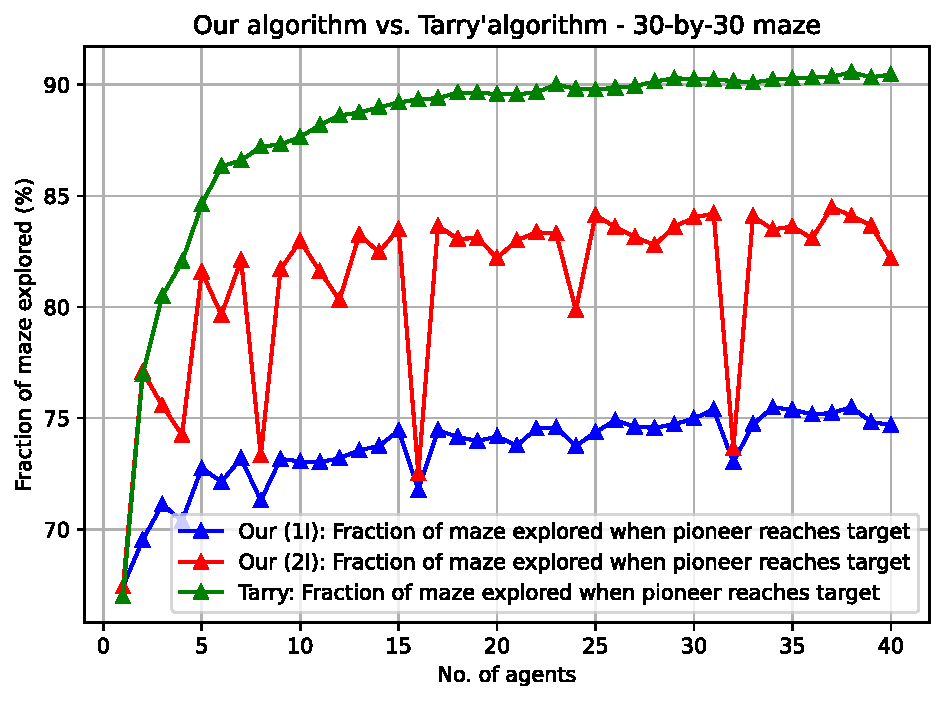
\includegraphics[width=.45\linewidth]{Cap3/our_algorithm_vs_tarry_algorithm/our_algorithm_vs_tarry_30x30_fraction.pdf} }}
    \qquad
    \subfloat[\centering $40 \times 40$maze]
    {{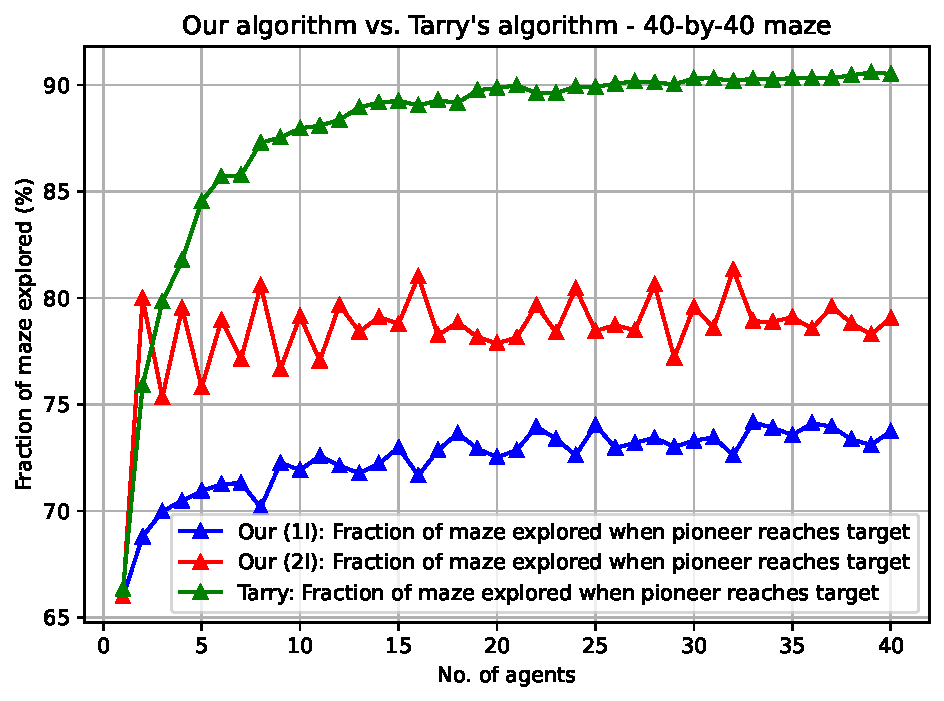
\includegraphics[width=.45\linewidth]{Cap3/our_algorithm_vs_tarry_algorithm/our_algorithm_vs_tarry_40x40_fraction.pdf} }}
    \caption{...}
    \label{our_algorithm_vs_tarry_fraction}
\end{figure}